\documentclass{acmtog}

\acmVolume{VV}
\acmNumber{N}
\acmYear{2012}
\acmMonth{February}
\acmArticleNum{XXX}  
\acmdoi{10.1145/XXXXXXX.YYYYYYY}

\usepackage{ucs}
\usepackage[utf8x]{inputenc}
\usepackage[english]{babel}


\usepackage[pdfborder={0 0 0}]{hyperref}
\usepackage{relsize}

\begin{document}

\markboth{Pedro Costa}{Fractal Based Terrain Generation}

\title{Terrain Generation using Fractals} % title

\author{Pedro Costa -- \texttt{pg19830@alunos.uminho.pt}
	\affil{University of Minho\\Department of Informatics}
}

\category{I.3.7}{Computer Graphics}{Three-Dimensional Graphics and Realism}[Fractals]
\category{I.3.5}{Computer Graphics}{Computational Geometry and Object Modeling}[Curve, surface, solid and object representations; Geometric algorithms, languages and systems]
\category{I.3.3}{Computer Graphics}{Picture/Image Generation}[Line and curve generation]
%\category{I.3.7}{Computer Graphics}{Three-Dimensional Graphics and Realism}[Animation]
%\category{I.3.5}{Computer Graphics}{Computational Geometry and Object Modeling}[Physically based modeling]

\terms{Algorithms, Theory}

\keywords{survey, state of the art, terrain generation}
%\keywords{Face animation, image-based modelling, iris animation, photorealism, physiologically-based modelling}

%\acmformat{Pamplona, V. F., Oliveira, M. M., and Baranoski, G. V. G. 2009. Photorealistic models for pupil light
%reflex and iridal pattern deformation.  {ACM Trans. Graph.} 28, 4, Article 106 (August 2009), 11 pages.\newline  DOI $=$
%10.1145/1559755.1559763\newline http://doi.acm.org/10.1145/1559755.1559763}

\maketitle

%\begin{bottomstuff} 
%Manuel M. Oliveira acknowledges a CNPq-Brazil fellowship (305613/2007-3). Gladimir V. G. Baranoski acknowledges a
%NSERC-Canada grant (238337). Microsoft Brazil provided additional support.
%
%Authors' addresses: land and/or email addresses.
%\end{bottomstuff}


\begin{abstract} 
The generation of terrains is a tool often necessary in many areas, such as military training, animation or game development. Creating such models manually is overwhelmingly complex and extracting detail from the real world generates massive quantities of data with limited detail.

Fractal based methods have evolved over decades and allow the procedural generation of very large terrains with few resources. The stochastic nature of fractals provide infinite possibilities for the final results, and pseudo-random number generators allow the creation of primitives with the required characteristics for virtual models.

This document presents the classical fractal methods for terrain generation, along with recent problems and trends such as the creation of water elements, the distribution of vegetation and the generation of cities and roads.
\end{abstract}



\section{Introduction}
Terrain generation has been a very important and deeply researched topic due to the wide variety of applications from military training to animation, with a special obvious impact in game development. The demand for new, unknown spaces in virtual environments is constant, and increasingly more exigent in realism. Manual modelling is not a viable option in these cases, as the processes, tools and techniques used are laborious, repetitive and often require speciallized 3D modelling skills.

Several approaches have been used to address this topic, but the usage of fractal geometry is a common ground where some of the best results have been achieved with relatively low effort. \cite{Belhadj07} divides most of the different used algorithms into three categories (some do not fall in any of these):
\begin{enumerate}
\item{Fractal-based methods, which are the scope of this document;}
\item{Fractal and physically based methods;}
\item{Physically based methods.}
\end{enumerate}

The fractal algorithms are generally faster, but rare are those which are able to create terrains according to fixed constraints. Some authors (\cite{Belhadj07}) make the distinction between geometric methods (\cite{Mandelbrot83,Fournier82,Miller86}) and procedural ones (\cite{Perlin85}) while others choose to consider every automatic generation process as a procedural approach (\cite{Smelik09}).

Similar work to the one done for this document has already been done recently in \cite{Smelik09}, with a high focus in modern trends. This document is primarily based on that work but adds more recent contributions (\cite{Chen11}), and digs deeper into the origins of this computer graphics branch. Although this field has been in development for more than three decades, the earlier works (\cite{Fournier82,Miller86}) are still heavily used and impose a requirement to understand newer approaches.

\section{Procedural Stochastic Modelling}
The usage of procedural modelling to generate virtual terrains has been an active research topic in computer graphics for more than thirty years. Instead of designing content by hand, procedural modelling allows the design of a procedure to automatically create the content. The applications are various and not restricted to the automatic generation of virtual spaces (such applications are out of the scope of this document though).

%from Fournier et al. 1982, fractal generated terrains as stochastic models
This field of research has been majorly focused on the random generation of terrains, either from scratch or constrained by the user. It is obvious that the randomness associated with this generation process can not be achieved with deterministic processes alone. Also due to their visual randomness, realistic natural objects can not be obtained with deterministic modelling. The number of samples required to achieve a visually acceptable model would easily create prohibitively large model databases, and the level of detail available would always be strictly binded to its size.

In their work, \cite{Fournier82} defined the formal concept of a stochastic model as a model where the object is represented by a sample path of some stochastic process of one or more variables. These models have three requirements:
\begin{enumerate}
\item{an appropriate object (or phenomenon) to be modeled;}
\item{a stochastic process to model it with;}
\item{an algorithm to compute the sample path of the process;}
\end{enumerate}
In the same document, the authors also identify a terrain as the example of an origin for a stochastic model. The processes associated with the models can be analitically defined. Therefore, many traditional algorithmic techniques, such as recursive subdivision, may be used to compute the required sample paths.

The recursive subdivision technique was introduced in \cite{Catmull78} for parametric patches, and the advantages are even more obvious in stochastic modelling, for two reasons:
\begin{itemize}
\item{It allows an infinite detail (one can always get more detail from the model), but at the same time, no more than the necessary detail is generated for a given scale;}
\item{The basis of the computation is an interpolation formula, which is, in general, much easier to compute than an incremental one, especially for midpoint interpolation.}
\end{itemize}

\subsection{Primitives}
Two properties required for a modelling primitive to be useful:
\begin{description}
\item[Internal consistency]{: the primitive must be reproducible in any position of an appropriate coordinate system at any level of detail, i.e., its features must not depend on its position and/or orientation in space;}
\item[External consistency]{: adjacent modelling primitives must provide continuity if a common boundary is to be shared.}
\end{description}

Both these properties are intuitively easy to preserve in deterministic modelling. Yet, in a stochastic modelling primitive these are more difficult to maintain and require more care in the design of generating algorithms.

\section{Fractals}
Natural 3-D terrain generally presents two features:
\begin{description}
\item[Infinite detail]{: the amount of detail captured by the vision system is the only limitation, as closer points of view will reveal smaller details;}
\item[Self-similarity]{: as one closes in, the details revealed in the terrain are similar to those shown at distance (the creases of a rock seen when very close it remind the ridges of mountains).}
\end{description}

These features are precisely those of fractal geometry. The generation of terrains based on fractals is a deeply studied subject, and is the basis of most modern approaches.

In the generation of a terrain, the presence of infinite detail can be obtained with the already mentioned recursive subdivision methods. At great distance, the amount of detail necessary is very small, resulting in a lower number of required polygons. When the distance decreases, new polygons can be generated in the required area by subdividing the polygons.

As for the self-similarity, \cite{MandelbrotVanNess1968} introduced the term ``fractional Brownian Motion'' (fBm) to denote a family of one-dimensional Gaussian stochastic processes which provide useful models for many natural time series. A sample of these functions may be observed at any scale, always showing the same statistical features. Thus, a surface generated using fBm would possess macroscopic features up to the order of magnitude of the overall surface generated, as well as arbitrarily small surface detail.

In \cite{Fournier82}, the authors used the fBm as the basis for their recursive subdivision algorithm. This algorithm starts from a limited domain and continuously subdivides it until a resolution threshold is reached. The image of a given point in the subdivided domain is then defined as the interpolation of the adjacent points (the first step uses the domain limits) displaced by a Gaussian function with zero mean and unit variance, with a constant seed. The influence of the generated displacement is decreased in each iteration. The decrease factor depends on a variable $h$ which controls the roughness of the result. To note that this algorithm has linear complexity, proportional to the number of points to be generated, with a rather small number of operations in each computation.

The application of Fournier's algorithm in two-dimensional primitives gives origin to three distinct algorithms: two based in polygon subdivision (for triangles and for quadrilaterals, respectively) and one for a stochastic parametric surface. For both the polygon subdivision cases, some care must be taken to ensure required properties of the modelling primitives. Internal consistency implies that the random number generated is independent of both the position and current scale. This requires the seeds of the random number generator to be indexed by some invariant identifier of the points rather than by any function dependent on their positions, and the random numbers to be generated in the same order at each level of the subdivision.

External consistency, on the other hand, implies the displacements for the points generated on a boundary shared by two polygons to be equal. This can be accomplished again by tying the seeds of the random number generator to the invariant point identifiers (making sure that the same identifiers are assigned to the corresponding points in the representation of each polygon's boundary). However, if the displacements are allowed to follow the polygon's normal, non coplanar polygons will cause discontinuities. The solution is to define a point's normal as the average of the normals of all the polygons containing it. Since this problem persists even for generated points which are completely internal to an original polygon, one can just assume the normal of the original polygon as the direction for the displacements.

\subsection{Algorithms}
The first algorithm presented in \cite{Fournier82} is meant for scenes in which all surfaces consist of triangles, and is known as the \textbf{triangular edge subdivision}. Each triangle can be subdivided into four smaller triangles by connecting the midpoints of each side, creating a pattern similar to a Sierpiński Sieve fractal (see \autoref{fig:fractal:sieve}). 

\begin{figure}[!htp]
	\begin{center}
		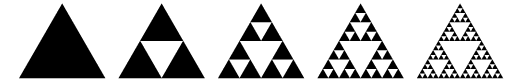
\includegraphics[width=\columnwidth]{images/fractals/sieve.png}
	\end{center}
	\caption{The Sierpiński Sieve fractal.\newline Source: \texttt{\url{http://mathworld.wolfram.com/SierpinskiSieve.html}}}
	\label{fig:fractal:sieve}
\end{figure}

With the same philosophy, the algorithm for quadrilaterals generates the midpoint of each side. Opposed midpoints are then connected, and the midpoints for both connections are generated. These two points are also connected, and the midpoint of this connection is taken to be the central point of the quadrilateral subdivision. The pattern created is also similar to a known fractal -- Sierpiński Carpet -- which can be seen in \autoref{fig:fractal:carpet}.

\begin{figure}[!htp]
	\begin{center}
		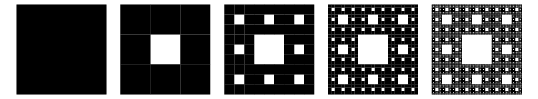
\includegraphics[width=\columnwidth]{images/fractals/carpet.png}
	\end{center}
	\caption{The Sierpiński Carpet fractal.\newline Source: \texttt{\url{http://mathworld.wolfram.com/SierpinskiCarpet.html}}}
	\label{fig:fractal:carpet}
\end{figure}

The stochastic parametric technique proposed by \cite{Fournier82}, also known as the \textbf{diamond-square subdivision}, is the basis of current algorithms, and is still used for the generation of terrain meshes with no constrains. The algorithm starts with the four corners of a quadrilateral terrain (usually a square) and works in two steps. First, in the diamond step, it generates the central point of the quadrilateral. This point is assumed to join four diamonds (in the first step, only half of each diamond is visible). Second, in the square step, the central point of each diamond is generated. All the points now form a grid of squares, and the process may be repeated until the required resolution is reached.

Gavin Miller, in \cite{Miller86}, describes the diamond-square algorithm as flawed. In his website\footnote{\texttt{\url{http://gameprogrammer.com/fractal.html}}}, Robert Pendleton explains that Miller's complains were due to the fact that he wanted to constrain the central point of the terrain -- if he left this point to be generated along with all the others, ``even he would've had to admit that the algorithm works pretty decently as a terrain generator''.

In his work, Miller provides an alternative to Fournier's algorithms. His alternative, which he calls \textbf{square-square subdivision} starts with a square base. The first step generates the points of a square with half the area of the original, with the same center. For each point, the value is taken to be in the proportion 9:3:3:1, where the nearer points have a greater weight in the interpolation. For each original square, the internal generated points are then connected to those of adjacent squares, resulting in a continuous. The first impression is that this algorithm wastes the border points of the original squares, but these will be useful in the next iteration, regaining use of the whole area.

\begin{figure}
	\begin{center}
		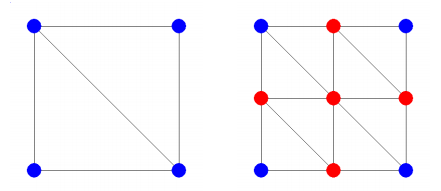
\includegraphics[width=\columnwidth]{images/algorithm/triangleedge.png}
	\end{center}
	\caption{One step of the triangle-edge subdivision. In blue, the original points. In red, the generated ones.}
	\label{fig:algorithm:tes}
\end{figure}

\begin{figure}
	\begin{center}
		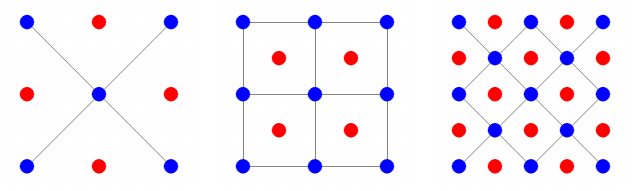
\includegraphics[width=\columnwidth]{images/algorithm/diamondsquare.png}
	\end{center}
	\caption{One full iteration of the diamond-square subdivision. For each step, the blue points are the originals and the red ones are the new generated points.}
	\label{fig:algorithm:dss}
\end{figure}

\begin{figure}
	\begin{center}
		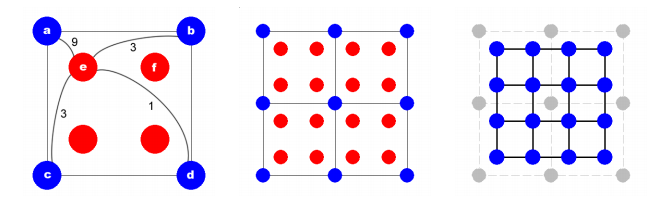
\includegraphics[width=\columnwidth]{images/algorithm/squaresquare.png}
	\end{center}
	\caption{One step of the square-square subdivision. In blue, the original points. In red, the generated ones.}
	\label{fig:algorithm:sss}
\end{figure}

\autoref{fig:algorithm:tes}, \autoref{fig:algorithm:dss} and \autoref{fig:algorithm:sss} contain the diagrams for the explained algorithms, taken from \cite{Macklem03}. Miller tested these three algorithms to generate constrained models where the four corners of the map and the central point are initialized. The results are presented in \autoref{fig:miller}.

\begin{figure}[!htp]
	\begin{center}
		\begin{enumerate}
		\item{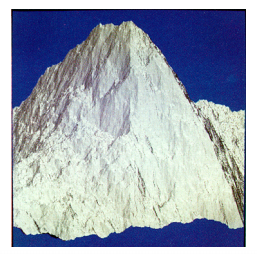
\includegraphics[width=0.7\columnwidth]{images/algorithm/triangleedge-mountain.png}\label{itm:tes}}
		\item{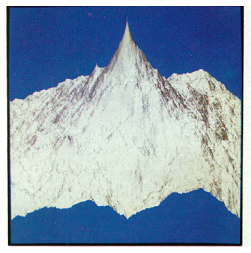
\includegraphics[width=0.7\columnwidth]{images/algorithm/diamondsquare-mountain.png}\label{itm:dss}}
		\item{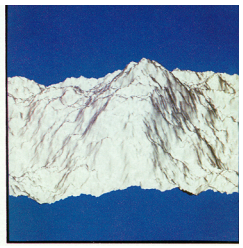
\includegraphics[width=0.7\columnwidth]{images/algorithm/squaresquare-mountain.png}\label{itm:sss}}
		\end{enumerate}
	\end{center}
	\caption{The same mountain generated with three different subdivision algorithms: (\ref{itm:tes}) was generated using triangle-edge subdivision, (\ref{itm:dss}) using the diamond-square subdivision and (\ref{itm:sss}) using square-square subdivision.}
	\label{fig:miller}
\end{figure}

Even nowadays, work is still being done to improve these algorithms. In \cite{Chen11}, the authors introduce the \textbf{BinSplit algorithm} based on the fBm and the fundamental principal of random midpoint displacement methods. It works like the triangle edge subdivision, but only the midpoint of the hypotenuse is generated, and only two new triangles are created.

\subsection{Perlin Noise}
In \cite{Perlin85}, Ken Perlin introduced a noise function based in a pseudo-random generator function. This function presented some interesting properties typical of fractal geometry. Since then, a common approach to terrain generation has also been to use this function to generate a gray-scale image, which can then be used as a height-map for the terrain.

\begin{figure}
	\begin{center}
		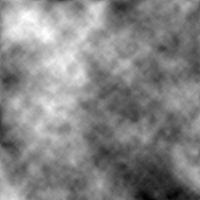
\includegraphics[width=0.6\columnwidth]{images/perlin.png}
	\end{center}
	\caption{Gray-scale image generated with Perlin's noise algorithm.\newline Source: \texttt{\url{http://nullprogram.com/img/noise/perlin.png}}}
	\label{fig:perlin}
\end{figure}

Perlin's algorithm for the noise function uses a $n$-dimensional grid ($n=2$ in this case). For each point $P$, it looks at each of the surrounding $2^{n}$ points $Q$ at a time. For each point $Q$, it generates a pseudo-random gradient vector $G$. It then computes the inner product $G \cdot ( P - Q )$. This will give the value at $P$ of the linear function with gradient $G$, which is zero at $Q$. Using $n$ weight curves, the final noise value for $P$ will be the interpolation between all the computed inner products.

Other noise functions exist to achieve diferent results, such as \textbf{cell noise} or \textbf{simplex noise}. A common practice is also to mix different noise functions.

\section{Transformations}
The height-maps generated with the presented methods can be transformed further using filters to optimize the landscape or to introduce physical phenomena simulations.

Filters are commonly used to optimize the generated terrain, for instance, smoothing the landscape. The method introduced by \cite{Chen11} is not very original and can be viewed as a slower version of the triangle edge subdivision, with a slightly lighter step, but the authors include a method to optimize any ocurrence of wrinkles and burrs. It consists in sweeping the entire mesh, and for each triangle, if the difference between one vertex and the other two is greater than a given threshold, the vertex with the higher value is lowered to the average value of the three.

As for physical phenomena, \cite{Olsen04} mentions two commonly used erosion algorithms: thermal and hydraulic. Thermal erosion diminishes sharp changes in the elevation by iteratively distributing the material from higher to lower points, until the maximum angle of stability for the material is reached. Hydraulic erosion algorithms simulate the phenomena of rainfall by using, for example, cellular automata, where the amount of water and dissolved material that flows out to other cells is calculated based on the local slope of the terrain surface. While these algorithms add great realism to the generated terrains, they are considerably slow, reason why recent research has focused in trying to port then to the GPU.

\begin{figure}[!htp]
	\begin{center}
		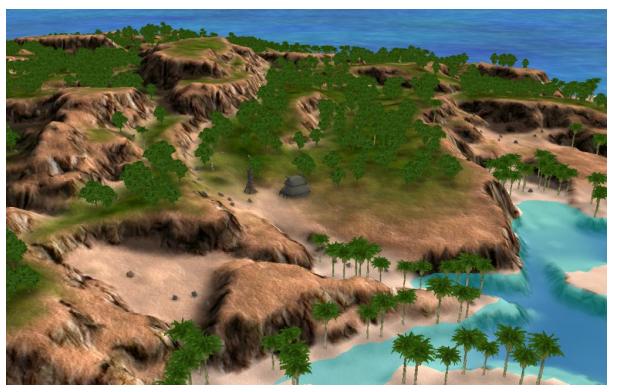
\includegraphics[width=\columnwidth]{images/erosion.png}
	\end{center}
	\caption{Screenshot from \textit{Tribal Trouble}, a realtime strategy game using the methods described in Olsen's paper for fast runtime generation of eroded terrain.}
\end{figure}

As previously mentioned, typical fractal based terrain generators rarely are able to deal with user constraints, which led to some specific research efforts on the topic. In \cite{Stachniak05}, the authors proposed a method which integrated constraints into the generation process using mask images. It employs a search algorithm that finds an acceptable set of deformations to apply to a random terrain in order to obtain a conforming one. In \cite{Schneider06}, the process explained is similar to the one of generation through noise functions, but the noise grid is replaced with a set of user-defined gray-scale images. In \cite{Zhou07}, the introduced technique generated a terrain based on an input height-map, followed by a user description of the lines representing large-scale features such as mountain ridges. \cite{Belhadj07} defines a system where a set of known elevation values (such as rivers and mountain ridges) constrain the midpoint displacement process.

\begin{figure}[!htp]
	\begin{center}
		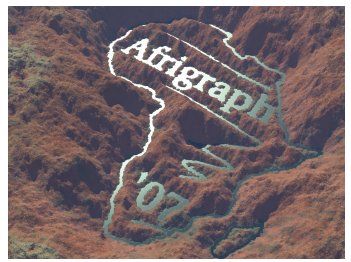
\includegraphics[width=\columnwidth]{images/constrained.png}
	\end{center}
	\caption{Realistic renderings of models generated using a user sketch as local constraints (from Belhadj, 2007)}
\end{figure}

An obvious limitation of all the terrain generation methods mentioned so far is that they are all unable to create overhangs and caves. All of these methods use some kind of function to translate a position into a height value, and a crucial property of every function is that there can be only one value for each given set of arguments. In a recent work, \cite{Peytavie09} provide a rather elaborate structure using different material layers which supports caves, arches and overhangs.

\subsection{Water}
Several algorithms have been proposed to address the generation of water elements in terrains, but this has received too little attention to the date, with the exception of rivers.

To generate rivers, the approaches are divided between those which run during and after the generation of the height-map. \cite{Kelley88} generates a stream network subdividing a single straight river, and then feeds it to the terrain generator which fills it using a scattered data interpolation function. \cite{Prusinkiewicz93} combine the height-map generation with the generation of a curved river. \cite{Belhadj05} on the other hand, works after the generation of the terrain, simulating the course of the river starting on mountain ridges.

Aside from rivers, water bodies tend to be created after the generation of the terrain using flood algorithms starting in low height points, but the results lack realism.

\subsection{L-Systems: Vegetation, Roads and Cities}

\begin{figure}[!htp]
	\begin{center}
		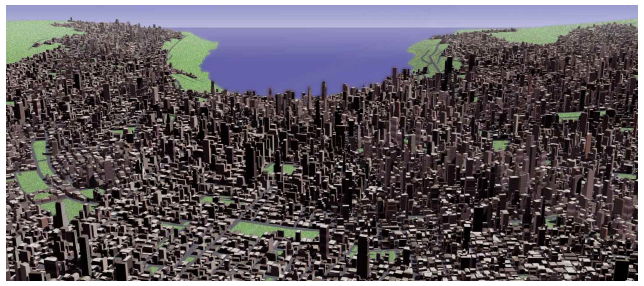
\includegraphics[width=\columnwidth]{images/city.png}
	\end{center}
	\caption{A virtual city modelled according to area of water, elevation and population density. The roads are created using goal-driven L-systems which try to connect high population density areas. Approximately 26000 buildings were created.}
\end{figure}

Lindenmayer-systems, an often user grammar rewriting system, are the choice of excellence for procedures which simulate the growth of plants. These processes start from the root, adding increasingly smaller branches and ending with leaves. \cite{Parish01} also use a goal-driven L-system to grow a road network, which tries to connect zones with high population density using specific road patterns (such as raster or the radial patterns). \cite{Wonka03} introduce the concept of split grammar, a formal context-free grammar, designed to create buildings which the authors use to create simple shape buildings with believable facades. \cite{Muller06} apply another type of grammar -- shape grammar. It uses context sensitive rules which allows the possibility to model roofs and rotated shapes.

Vegetation distribution mechanisms are often used after defining the plants, to save the modellers the laborious task of manually placing every model individually in large areas (such as a forest). \cite{Deussen98} describe a model which simulates an ecosystem. This takes the generated terrain and a water network map as input and uses the available information about the plants (such as rate of growth) to iteratively compute their distribution according to rules such as the competition for soil, sunlight and water, resulting in a very slow process.

\begin{figure}[!htp]
	\begin{center}
		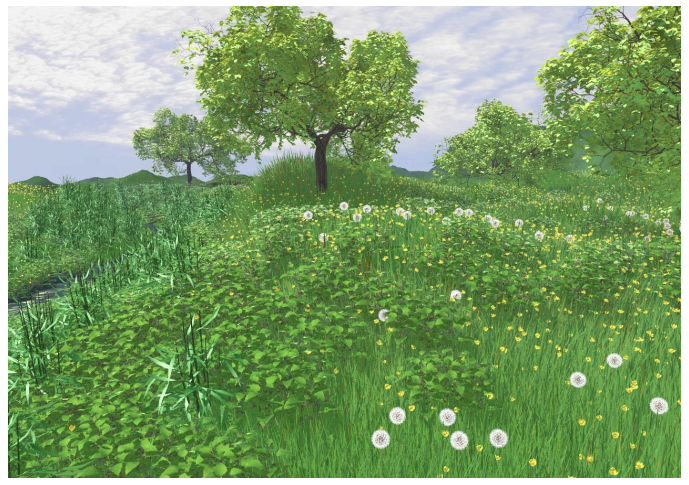
\includegraphics[width=\columnwidth]{images/ecosys.png}
	\end{center}
	\caption{A scene created using the work of Deussen et al., 1998. Plants are placed iteratively according to soil, water and sunlight competition rules.}
\end{figure}

Road networks are usually created using real world based patterns or L-systems, but different approaches have been researched to obtain high levels of realism. \cite{Lechner03} went for a agent-based approach in a city divided into different areas (such as residential, commercial, industrial, etc), where one agent would search for unconnected areas in the city, reaching for it in the most suitable path if such an area is not located too far from the already existing road, and one which is placed in random locations of the existing network, directly connects it to a random location if the travel time through the shortest path to that spot is considered excessive. Other approaches rely on the terrain profile. \cite{Kelly07} plan the path of the main roads between user set nodes to maintain an even change in the elevation, as much as possible. \cite{Bruneton08} propose a method to blend road profiles into the height-map using shaders.

Although L-systems can be used to successfully create buildings, the cities created by these methods lack a realistic structure. \cite{Groenewegen09} generate the distribuition of different types of districts according to land use models of known cities, taking into account relevant factors (such as the historic core of the city and the attraction of the terrain for each kind of area). \cite{Weber09} use comparable models in a simplified simulation of expanding cities, which results in a relatively fast and interactive system.

\begin{figure}[!htp]
	\begin{center}
		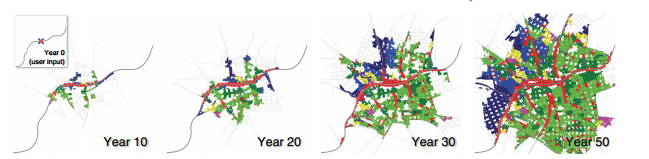
\includegraphics[width=\columnwidth]{images/citytime.png}
	\end{center}
	\caption{Example simulation of a city on a given street. The initial configuration is defined by the user. Different colors are used for distinct purpose land lots. To be noted, the blue ones represent industrial zones, which are reallocated over the years.}
\end{figure}

\section{Conclusion}
This document presented the overall process of terrain generation, where a special importance was given to fractal based methods. It began with a formal explanation of classical concepts regarding procedural stochastic modeling, where terms the requirements for stochastic models were defined, followed by the required properties for any modeling primitive, which are especially difficult to achieve using stochastic models.

The origins of fractal based methods were explained, along with some history of fractal theory. The three first algorithms used for the mesh generation process, still in the heart of modern approaches, were explained. The fractal noise methods were also covered, with a brief explanation of Perlin's noise algorithm.

Concluded the mesh, several approaches for transformations were discussed. These intended to achieve better realism, either by including other elements present in typical landscapes of the real world, such as rivers and vegetation, or by generating human related terrain elements, like roads and cities. Several approaches to various problems were mentioned. A special focus was given to solutions using L-Systems, due to being closely related to fractals.

During the last thirty years, the topic of terrain generation, more specifically fractal based methods, has evolved greatly from simple mesh generators to complex landscape builders. The number of references used throughout this document is a sign of how widely researched this theme is. At the same time, current state of the art clearly shows that some areas (especially, water bodies generation) still require a lot of work and have plenty of space for maturing.

The work done for this document is far from complete, as it lacks deep detail in most of the modern approaches. However, even after all the effort put into understanding the basis of these methods, which showed more than four decades of material, deeper investigation is also required to better understand, for example, the noise mechanisms. Still, given the time contraints and the purpose of this document, the information included easily provides any reader with the required knowledge in terrain generation.

\bibliographystyle{acmtog}
\bibliography{mono}

\end{document}
